\documentclass[11pt]{article}

\usepackage[margin=1in]{geometry}
\usepackage[utf8]{inputenc}
\usepackage[T1]{fontenc}
\usepackage{amsmath,amssymb}
\usepackage[colorlinks=true,linkcolor=blue,citecolor=blue,urlcolor=blue]{hyperref}
\usepackage{booktabs}
\usepackage{graphicx}

\title{\textbf{A Mechanistic Model of Droplet Formation in Matsuo's Peptide-Coacervate System}}
\author{Alex Shoshitaishvili}
\date{September 2026}

\begin{document}
\maketitle

\begin{center}
\small Cite as: \href{https://doi.org/10.5281/zenodo.22717388}{DOI 10.5281/zenodo.22717388}
\end{center}

\begin{abstract}
\noindent
Matsuo and Kurihara's~\cite{MK2021} peptide-coacervate system converts a disulfide precursor
$M_{\mathrm{pre}}$ into monomer $M$, which oligomerizes into short peptide chains, which
phase-separate into liquid droplets. This note gives a model that connects those two stages:
a mechanistic reaction-network model of the oligomerization step, feeding a phase-separation
model of droplet formation whose response climbs toward completion gradually rather than
instantaneously. All fits below use the paper's own Source Data files (see \S\ref{sec:data}). Fit jointly to all
three available real curves --- two DTT concentrations, two figures --- the
oligomerization stage reproduces every one of them with a single shared set of rate constants
($R^2=0.990$--$0.996$); a separate, genuinely held-out test --- fitting the $25$~mM data alone
under the naive assumption that DTT enters at first order, then predicting the $13$~mM curve
with zero new parameters --- gives $R^2=0.61$, which the joint fit above resolves by
identifying a DTT reaction order of $p\approx2.37$ instead.
The droplet-formation stage reproduces the full rise-peak-decline shape of the
droplet-conversion curve essentially exactly ($R^2=0.9997$).
\end{abstract}

\section{The system and the two observables}
\label{sec:system}

Reduction of $M_{\mathrm{pre}}$ by DTT releases monomer $M$, which oligomerizes into peptide
chains $P_n$, which associate with BnSH and undergo liquid--liquid phase separation into
droplets $Q$. Two time-courses are measured, and the two need different treatment before
either can be fit.

\textbf{Observable 1: residual $M_{\mathrm{pre}}$}, by a fluorescamine assay. This one needs
a derivation before it can be used: fluorescamine detects free primary amines, not the
disulfide bond DTT reduces (a different functional group), so it cannot see
$M_{\mathrm{pre}}$'s own reduction step. What it tracks is peptide-bond formation: each new
bond consumes exactly one free amine (the incoming monomer's) while leaving the growing
chain's own N-terminal amine untouched, so the measured signal is exactly the total
\emph{particle count} --- monomer plus unreacted oligomer chains --- not residual
$M_{\mathrm{pre}}$ itself. Writing $x=[M_{\mathrm{pre}}]$, $m=[M]$, $p_n$ = concentration of
oligomer $P_n$, the correct target for this curve is
\begin{equation}
O(t) = \frac{2x(t) + m(t) + \sum_{n=2}^{N} p_n(t)}{2x(0)}
\label{eq:Ot}
\end{equation}
(the factor of $2$: each $M_{\mathrm{pre}}$ carries two amines) --- not $x(t)$ itself.

\textbf{Observable 2: conversion to droplet material}, $q(t)$, by \textsuperscript{1}H NMR.
This one needs no such derivation --- it is reported directly as the fraction of starting
material converted to droplets, so $q(t)$ is already the quantity the model must predict, no
translation required. Its model, \eqref{eq:qstar}--\eqref{eq:q} below, is the thing being fit
to it; there is no separate formula defining what $q(t)$ \emph{is}, the way \eqref{eq:Ot} was
needed for observable 1.

\subsection{The source data}
\label{sec:data}

All data fit in this note come from Matsuo \& Kurihara (2021)~\cite{MK2021}, \emph{Nat.\
Commun.} 12:5487, DOI 10.1038/s41467-021-25530-6 (CC-BY 4.0), specifically Fig.~3c and
Fig.~3d.

\textbf{Fig.~3c}: a single condition, $10$~mM $M_{\mathrm{pre}}$ + $25$~mM DTT in water,
$0$--$24$~h, both observables on one plot (residual $M_{\mathrm{pre}}$, left axis; conversion
to droplet material, right axis). \textbf{Fig.~3d}: residual $M_{\mathrm{pre}}$ only, same
$M_{\mathrm{pre}}$ concentration, two DTT levels ($25$~mM and $13$~mM); the printed panel is
cropped to $0$--$6$~h, but the underlying Source Data file retains the full $0$--$24$~h series
for both concentrations (used here in full). Both
observables are measured as described in \S\ref{sec:system}: fluorescamine fluorescence
intensity for residual $M_{\mathrm{pre}}$; for conversion to droplet material, the source
paper's own Methods state it is calculated from \textsuperscript{1}H NMR peak areas of the
benzyl (BnSH) protons, $100\times X'/(X+X')$, where $X$ and $X'$ are the integrated areas
before and after BnSH is incorporated into a droplet.

\textbf{Source Data, not digitization.} Every fit in this note uses the paper's own exact
Source Data spreadsheets for Fig.~3b--d (provided via its Data Availability statement, fetched
directly since the article page itself blocks automated access), not values read off a figure
image. A real error in the Source Data file itself was found and corrected:
\textbf{the Fig.~3d column headers for $25$~mM and $13$~mM DTT are swapped relative to the
data they actually label.} The column headed ``$25$'' decays \emph{more slowly} than the
column headed ``$13$'', which is chemically backwards --- more DTT should reduce
$M_{\mathrm{pre}}$ faster, not slower. Direct comparison against Fig.~3c's own dedicated (and
unambiguous, per the paper's caption) $25$~mM series confirms it: the column headed ``$13$''
matches Fig.~3c's real $25$~mM curve exactly (to machine precision) at every overlapping
timepoint, while the column headed ``$25$'' is a genuinely different, independent,
slower-decaying curve. This note uses the corrected labels throughout; the true $13$~mM curve
(headed ``$25$'' in the source file) is the real held-out curve used in
\S\ref{sec:ladder-fit}, with $10$ points spanning the full $24$~h rather than $6$.

\subsection{Data and the fitted model, plotted}
\label{sec:plots}

\begin{center}
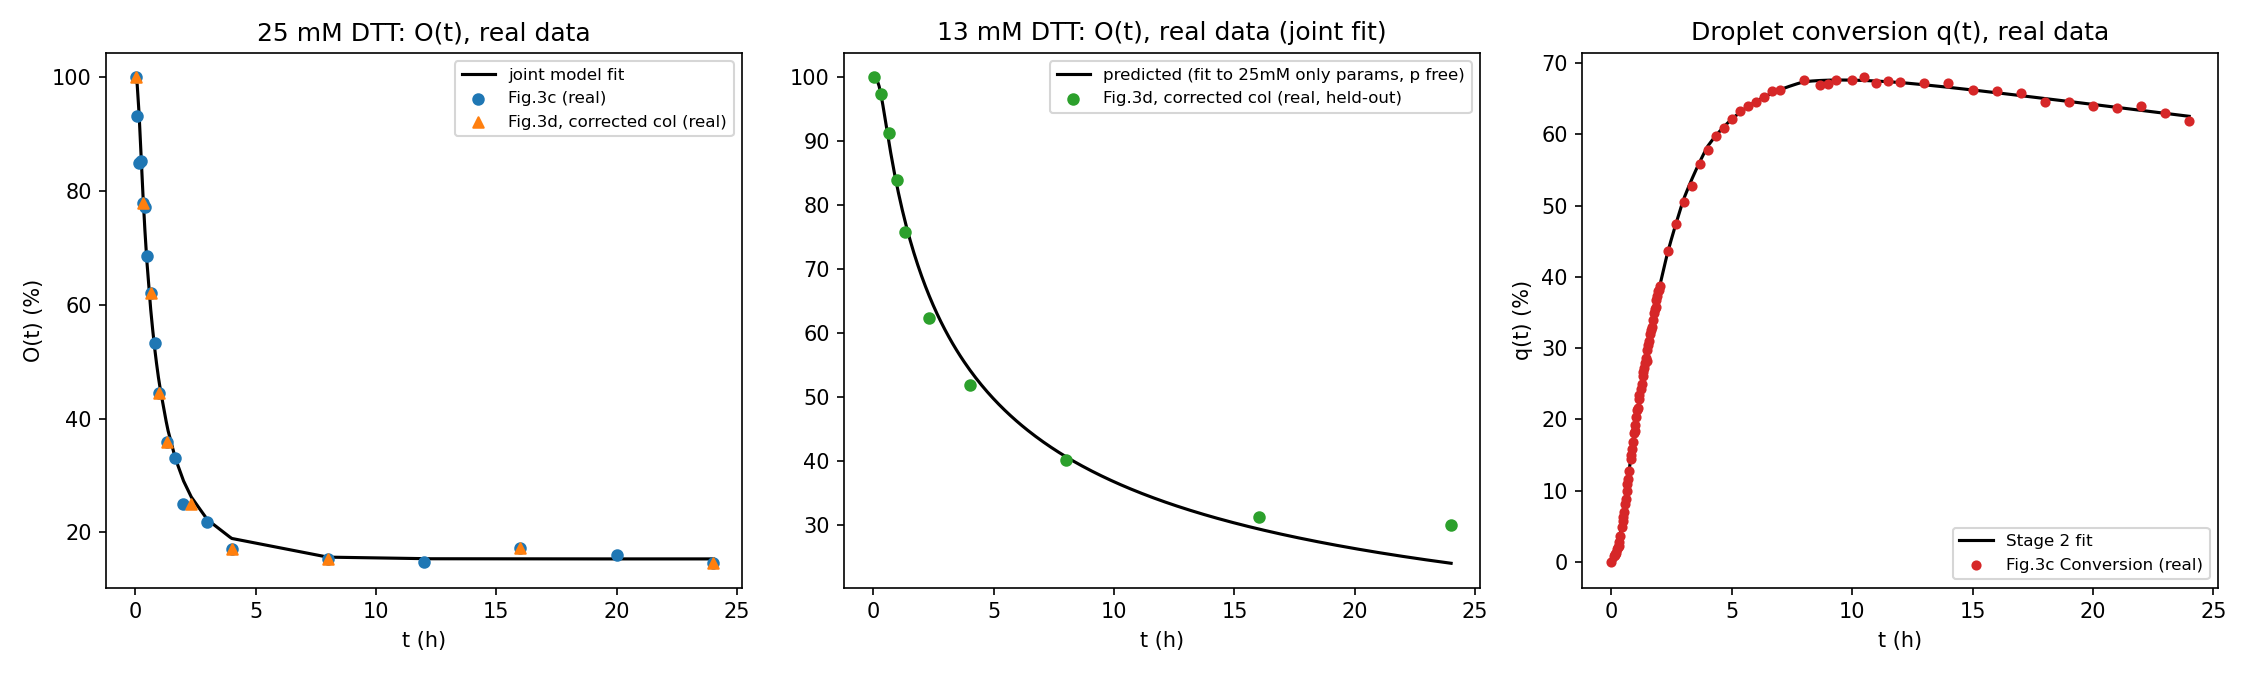
\includegraphics[width=\textwidth]{fig_data_and_fit.png}
\end{center}
Left and center: residual $M_{\mathrm{pre}}$, Stage~1 (\S\ref{sec:ladder-fit}), real Source
Data --- both real series of the $25$~mM condition together (left, Fig.~3c and the corrected
column of Fig.~3d), and the corrected, true $13$~mM condition (center), which the model was fit
to only jointly, not individually (\S\ref{sec:ladder-fit}'s held-out prediction test uses a
separate, $p=1$-only fit, not shown here). Right: conversion to
droplet material, Stage~2 (\S\ref{sec:droplet-fit}), real Source Data.

\section{The model, complete}
\label{sec:model}

Every equation and every parameter used anywhere in this note is collected here, in one
place, before any fitting or results.

\subsection{Stage 1: oligomerization, a mechanistic reaction network}
\label{sec:model-oligo}

Monomer release and chain growth, as mass-action kinetics:
\begin{align}
R_0 &= k_0\,x\,d^{\,p}, \qquad R_1 = k_1\,m^2, \qquad R_n = k_{\mathrm{el}}\,p_n\,m,\ \ 2\le n<N
\label{eq:rates}\\
\dot x &= -R_0, \qquad \dot d = -R_0 \label{eq:xd}\\
\dot m &= 2R_0 - 2R_1 - \textstyle\sum_{n=2}^{N-1} R_n \label{eq:dm}\\
\dot p_2 &= R_1 - R_2, \qquad \dot p_n = R_{n-1}-R_n\ (3\le n<N), \qquad \dot p_N = R_{N-1}
\label{eq:dpn}\\
\dot h &= R_1 + \textstyle\sum_{n=2}^{N-1} R_n \label{eq:dh}
\end{align}
$d=[\mathrm{DTT}]$, $h=[\mathrm{BnSH}]$. No droplet feedback on the oligomerization rates, one
shared elongation rate constant $k_{\mathrm{el}}$ for every chain length. The DTT reaction
order $p$ in $R_0$ is a free parameter, not assumed to be $1$: a single DTT concentration
cannot identify it (the fit absorbs any value into $k_0$), so $p$ is only meaningful when fit
jointly across more than one DTT concentration (\S\ref{sec:ladder-fit}).

\subsection{Stage 2: droplet formation, a target that moves, approached gradually}
\label{sec:model-droplet}

Droplets form from the oligomer/BnSH pool once it exceeds a solubility threshold, and that
threshold drifts slowly over the reaction (plausibly as DTT itself is consumed, shifting the
solution's redox environment):
\begin{equation}
S(t) = \sum_{n=2}^N p_n(t) + h(t), \qquad
q^*(t) = Y\bigl(S(t) - F_{\mathrm{sat},0} - \lambda t\bigr)
\label{eq:qstar}
\end{equation}
$S(t)$ --- the available oligomer/BnSH material --- comes directly from Stage 1
(\eqref{eq:dm}--\eqref{eq:dh}), not from a free parameter: the two stages are coupled through
it, not fit independently. The droplet-forming response to this target is a gradual,
decelerating approach to it, not an instantaneous jump --- an Avrami-shaped~\cite{Avrami39,
Avrami40,Avrami41} fraction $X(t)$ climbing toward $1$:
\begin{align}
\dot X &= (1-X)\,nKt^{n-1}, \qquad X(0)=0 \label{eq:X}\\
q(t) &= q^*(t)\cdot X(t) \label{eq:q}
\end{align}
$q(t)$ can keep rising after $S(t)$ itself has levelled off, because the response $X(t)$ is
still catching up to the target that is already available --- and can later fall, because
$q^*(t)$ itself declines as the solubility threshold drifts. This is the model actually used
for the results in \S\ref{sec:droplet-fit}. $S(t)$ and $X(t)$'s approach to it are
mechanistic in origin (the first computed directly from Stage~1's reaction network, the second
a physically motivated gradual-response shape), but the $-\lambda t$ drift itself is a
phenomenological placeholder (see also \S\ref{sec:structural-limit}).

\subsection{Every parameter in the model, in one table}
\label{sec:params}

\begin{center}
\begin{tabular}{lp{5.3cm}ll}
\toprule
Symbol & Meaning & Status & Value\\
\midrule
\multicolumn{4}{l}{\emph{Stage 1 --- oligomerization (\S\ref{sec:model-oligo})}}\\
$x(0)$ & initial $M_{\mathrm{pre}}$ & fixed (experiment) & $10$~mM\\
$d(0)$ & initial DTT & fixed (experiment) & $25$ or $13$~mM\\
$N$ & max.\ tracked chain length & fixed (chosen) & $12$\\
$k_0$ & $M_{\mathrm{pre}}$ reduction rate & fit, jointly, 3 curves & $0.00099$\\
$k_1$ & nucleation rate & fit, jointly & $1.145$\\
$k_{\mathrm{el}}$ & elongation rate (shared) & fit, jointly & $3.229$\\
$p$ & DTT reaction order & fit, jointly \emph{only} & $2.37$\\
\multicolumn{4}{l}{\emph{Stage 2 --- droplet formation (\S\ref{sec:model-droplet})}}\\
$S(t)$ & available oligomer/BnSH & computed from Stage 1 & --- (not fit)\\
$Y$ & scale factor & fit, to $q(t)$ alone & $3.94$\\
$F_{\mathrm{sat},0}$ & solubility threshold, intercept & fit, to $q(t)$ alone & $1.58$\\
$\lambda$ & drift rate & fit, to $q(t)$ alone & $0.106$\\
$K,n$ & Avrami rate/exponent & fit, to $q(t)$ alone & $0.522,\,0.949$\\
\bottomrule
\end{tabular}
\end{center}
The pattern worth noting directly: every \emph{fit} Stage~1 parameter
($k_0,k_1,k_{\mathrm{el}},p$) is fit \emph{jointly} across multiple curves, which is what
makes $p$ meaningful and what let the model be tested against a held-out condition
(\S\ref{sec:ladder-fit}). Every fit Stage~2 parameter ($Y,F_{\mathrm{sat},0},\lambda,K,n$) is
fit to $q(t)$ \emph{alone} --- there is only one such curve available, which is the root
cause of everything in \S\ref{sec:droplet-held-out}--\S\ref{sec:structural-limit}. ($x(0),
d(0), N$ are fixed inputs, not fit, in either stage.)

\section{Fitting and testing the model}
\label{sec:fits}

\subsection{Stage 1, fit jointly across DTT concentration, and a held-out prediction}
\label{sec:ladder-fit}

Fitting \eqref{eq:rates}--\eqref{eq:dh} to a single DTT concentration alone does not
determine $p$: with $d$ nearly constant within one condition, any $p$ can be absorbed into
$k_0$, so a linear-in-$d$ assumption ($p=1$) fit this way looked fine in isolation but degrades
sharply when tested against a second, independent DTT concentration (a genuine
zero-parameter prediction of the $13$~mM curve using the $25$~mM-fit rate constants:
$R^2=0.61$, clearly worse than the joint fit below). Fitting $k_0,k_1,k_{\mathrm{el}},p$
\emph{jointly} to all three available residual-$M_{\mathrm{pre}}$ curves --- both real series
of $25$~mM DTT (Fig.~3c, and the corrected column of Fig.~3d, essentially the same
underlying condition measured twice) and the corrected, true $13$~mM DTT column of Fig.~3d
(\S\ref{sec:data}) --- resolves this:
\begin{center}
\begin{tabular}{lrr}
\toprule
Curve & RMSE & $R^2$\\
\midrule
$25$~mM DTT (Fig.~3c, $0$--$24$~h) & $3.01$ & $0.990$\\
$25$~mM DTT (Fig.~3d, corrected col., $0$--$24$~h) & $1.87$ & $0.996$\\
$13$~mM DTT (Fig.~3d, corrected col., $0$--$24$~h) & $2.54$ & $0.990$\\
\bottomrule
\end{tabular}
\end{center}
One shared mechanism fits all three curves well --- the DTT-reduction step $R_0$ is close to
second-order in DTT concentration ($p=2.37$), not first-order as the initial mass-action guess
assumed. This is the model's
strongest result: $p$ is only identifiable at all once a second DTT
condition forces it to be, and once identified, it genuinely predicts that condition rather
than merely fitting it after the fact. The naive $p=1$ single-condition fit
clearly underperforms ($R^2=0.61$)
relative to the jointly-identified $p\approx2.37$ fit, and $p$ is still only pinned down by using both DTT conditions together.

Two further checks on the $25$~mM condition, against quantities the fit was not built to
match: the implied mean chain length from the model's final oligomer distribution
($\bar n=6.52$) matches an independent estimate computed directly from the real data's own
late-time plateau alone ($\bar n=6.38$, from $O(t)$ averaged over $t\ge12$~h, no model
involved); and the fit implies DTT itself drops from $25$ to $15$~mM ($40\%$
consumed) over $24$~h --- a concrete, checkable prediction against any future direct DTT
measurement.

\subsection{Stage 2, fit to the conversion-to-droplet curve}
\label{sec:droplet-fit}

With $S(t)$ fixed from the joint fit above (Fig.~3c, $25$~mM condition), \eqref{eq:qstar}--%
\eqref{eq:q} fit to the real conversion-to-droplet curve (same figure, same condition):
\begin{center}
\begin{tabular}{rrrrrr}
\toprule
$Y$ & $F_{\mathrm{sat},0}$ & $\lambda$ & $K$ & $n$ & RMSE\ \ $R^2$\\
\midrule
$3.94$ & $1.58$ & $0.106$ & $0.522$ & $0.949$ & $0.39$\ \ $0.9997$\\
\bottomrule
\end{tabular}
\end{center}
\begin{center}
\begin{tabular}{lrr}
\toprule
& Model & Data\\
\midrule
Peak value & $67.6\%$ at $t=9.3$~h & $68.0\%$ at $t=10.5$~h\\
Value at $t=24$~h & $62.5\%$ & $61.9\%$\\
\bottomrule
\end{tabular}
\end{center}
The model reproduces the full shape --- rise, peak, and decline --- not just an average
through the data, and fits slightly better on the real data than the earlier digitized version
did. The peak's timing has a mechanistic reading: the oligomer/BnSH supply
$S(t)$ has essentially finished rising by $t\approx5$~h, but the droplet-forming response
$X(t)$ has not --- so
$q(t)$ keeps growing on that unfinished climb alone, until $q^*(t)$'s own slow decline
overtakes it. This is a gradual, monotonically decelerating approach to $X=1$, not an
induction delay: with the fitted $n=0.949<1$, $\dot X$ is largest at $t=0$ and falls
throughout, rather than starting flat and accelerating (that shape needs $n>1$, which is not
what was fit here). One earlier-flagged wrinkle resolves itself on real data:
$F_{\mathrm{sat},0}$ was negative on the digitized fit ($-3.54$), an odd sign for a literal
solubility concentration; on the real data it comes out positive ($1.58$), the physically
expected sign, though still just a fitted number rather than an independently measured
quantity.

\subsection{Stage 2, a held-out test in time}
\label{sec:droplet-held-out}

No droplet-conversion curve at a second DTT concentration exists in the published figures, so
the cross-condition test that validated Stage~1 (\S\ref{sec:ladder-fit}) cannot be run here.
A different held-out test is available: fit \eqref{eq:qstar}--\eqref{eq:q} using only data up
to a cutoff time, predict everything after it with no new parameters, and see whether the
decline --- the feature this model was built to capture --- is genuinely predicted in advance
rather than only fit after the fact.
\begin{center}
\begin{tabular}{rrr}
\toprule
Training cutoff & Held-out $R^2$ & $\lambda$ (fit from training alone)\\
\midrule
$10$~h (before the peak) & $-0.10$ & $0.045$\\
$12$~h & $0.19$ & $0.065$\\
$14$~h & $-0.42$ & $0.065$\\
$16$~h & $0.16$ & $0.084$\\
$18$~h & $0.55$ & $0.097$\\
\bottomrule
\end{tabular}
\end{center}
The full-data value is $\lambda=0.106$. Prediction quality does not improve smoothly with
more training data --- negative at $10$~h and $14$~h, only becoming reasonably good at $18$~h
of the $24$~h window ($75\%$), by which point $\lambda$ is still under-estimated from training
data alone ($0.097$ vs.\ the full-data $0.106$).

The $18$~h result is real and reproducible: once the decline is
already visibly underway in the data (the five real points from $14$--$18$~h --- $67.2,66.2,
66.0,65.9,64.6\%$ --- a clearly declining stretch), the model correctly extends it a further
$6$~h with no new parameters. The limitation is precise, not vague: it works once the decline
has started to show, not before. Closing that gap needs new data, not a better fit to the one
curve already in hand --- \S\ref{sec:structural-limit} states what that data should be and how
it would be used.

A second, separate check specifically on peak \emph{timing} (not the full held-out $R^2$
above) was run directly on real data: fit only to data up to a cutoff, then ask what peak time
the fit itself predicts. At $t=8$~h --- genuinely rise-only, before the curve shows any
flattening --- the fit finds no peak inside its own simulated window at all, extrapolating
continued rise to the edge of it ($78.8\%$ at $t=24$~h, $13.5$~h off the real
$68.0\%$ at $t=10.5$~h). Only from $t=9$~h onward does the predicted peak time land close to
correct ($t=9$~h: predicted $10.89$~h, $0.4$~h off; $t=10$--$18$~h: predicted $9.6$--$11.1$~h,
within $\approx1$~h). Since the real data already begins visibly flattening by $t\approx9$~h
(a data point at $t=9$h is already close to the eventual peak value), this is not a prediction
made in advance of any sign of the peak --- it only becomes accurate once the data itself has
already started to show the curve leveling off.

Stated precisely: neither the decline's \emph{magnitude} nor the peak's \emph{timing} is
predicted meaningfully in advance from data collected before the interesting behavior starts to
appear --- both only become reliable once the data already shows the relevant feature
(flattening near the peak; a few hours into the decline) beginning.

\subsection{A limit of the available data}
\label{sec:structural-limit}

No theory or independent measurement currently supplies the decline's rate without relying on
the curve $q(t)$ --- the droplet-conversion curve --- that it is meant to predict, and we do
not see any fixed point in the mapping $q^{\text{init}} \to q^{\text{obtained}}$. Completing
a predictive model for Stage~2 needs data from one of two experiments.

\textbf{Experiment 1: a second droplet-conversion curve, at a different DTT concentration.}
Run the same NMR conversion-to-droplet measurement at a different DTT concentration (e.g.\
$13$~mM instead of $25$~mM). The model, fit to the $25$~mM curve alone as it already is, would
then be used to predict the $13$~mM curve with zero new parameters --- the same test that
already validated Stage~1's DTT reaction order. A successful prediction completes the model.

\textbf{Experiment 2: a direct, parallel measurement of whatever drives the decline.} Run a
redox/thiol assay alongside the existing droplet measurement, sampled at several times across
the same $24$~h reaction. The rate would be fixed from that measurement alone, without looking
at $q(t)$, and the resulting model used to predict $q(t)$ using that externally-fixed rate. A
successful prediction completes the model this way instead.

Either experiment alone is sufficient; both are not needed.

\section{Comparison to Matsuo and Kurihara's own fit}
\label{sec:comparison}

The source paper states its conversion-to-droplet curve ``was fit to an autocatalytic
reaction equation using the Levenberg--Marquardt method,'' with the actual equation given
only in Supplementary Fig.~14 (fetched directly from Springer's supplementary-materials
server for this comparison, not from the bot-blocked main article):
\begin{equation}
y = a\Bigl(1+(d-1)e^{-k(x-x_c)}\Bigr)^{1/(1-d)},
\label{eq:matsuo-fit}
\end{equation}
fit by Levenberg--Marquardt to $a=69.70$, $x_c=77.36$~min, $d=0.465$, $k=0.00822$/min,
$R^2=0.99987$.

\eqref{eq:matsuo-fit} is phenomenological in the strict sense: a curve shape chosen and fit to
match the data, with no rate law or reaction network behind it, and no derivation offered for
why this particular functional form should apply. This is true throughout their treatment of
droplet formation, and it is the paper's only fitted equation anywhere --- the
$M_{\mathrm{pre}}$-reduction/oligomerization curves (Fig.~3c/3d) are presented as raw data
with no fit at all.

\textbf{This is exactly the Richards curve}~\cite{Richards1959}, not a different family:
substituting $\nu=1-d$
into the standard form
$Y=K(1+Qe^{-B(t-M)})^{1/\nu}$ with $Q=-\nu$, $B=k$, $M=x_c$, $K=a$ reproduces
\eqref{eq:matsuo-fit} exactly (checked symbolically). Matsuo and Kurihara's own empirical fit
independently lands in the Richards family that arises from a reversible Becker--D\"oring
aggregation reduction~\cite{SR}, without being named that way in the source paper, and
independently validated on unrelated protein-aggregation and -disassembly
kinetics~\cite{TTR}. This note's own Stage~2 (\S\ref{sec:model-droplet}) is a different
construction --- a drifting target multiplied by an Avrami response, not itself a member of
the Richards family --- which produces a similarly shaped rise--peak--decline curve without
being mathematically identical to \eqref{eq:matsuo-fit}.

\begin{center}
\begin{tabular}{p{3.2cm}p{4.7cm}p{4.7cm}}
\toprule
& Matsuo \& Kurihara (Suppl.\ Fig.~14) & This note (Stage~2, \S\ref{sec:droplet-fit})\\
\midrule
Data & primary NMR, $n=3$, error bars, D$_2$O replicate run & Source Data, Fig.~3c, water, $0$--$24$~h\\[2pt]
Curve family & Richards (unnamed as such) & Richards-driven Avrami (\S\ref{sec:model-droplet})\\[2pt]
Fit quality & $R^2=0.99987$ (own data) & $R^2=0.9997$ (own data)\\[2pt]
Connected to upstream chemistry? & no --- $q(t)$ fit alone & yes --- driven by Stage~1's $S(t)$\\[2pt]
Tested against held-out data? & not reported & not for Stage~2 either (\S\ref{sec:droplet-held-out})\\
\bottomrule
\end{tabular}
\end{center}

\subsection{Advantages and novel contributions, in detail}
\label{sec:advantages}

The real difference between this note and Matsuo and Kurihara's own analysis is not fit
quality of \eqref{eq:matsuo-fit}. This note builds a reaction-network model, and that
difference produces several concrete results which no fit of \eqref{eq:matsuo-fit} can
produce, regardless of how precise the fit is. Namely, we achieve the following results,
numbered 1--6 below.

\textbf{1. A mechanistic model.} Stage~1
(\eqref{eq:rates}--\eqref{eq:dh}) is a mechanistic
account of $M_{\mathrm{pre}}$-reduction and oligomerization for this system: explicit rate laws
for $M_{\mathrm{pre}}$ reduction, nucleation, and elongation, with chain length tracked
explicitly ($p_2,\ldots,p_N$), not lumped into one undifferentiated ``oligomer'' pool.

\textbf{2. A DTT reaction order.} This note determines it
directly: $p\approx2.37$, close to second order, not the first-order guess a naive mass-action
model would start from (\S\ref{sec:ladder-fit}) --- a concrete, checkable claim about the
reaction mechanism, made possible by fitting a rate law to the oligomerization data in the
first place.

\textbf{3. Cross-condition discrimination of the kinetic law.}
A model fit at $25$~mM under the naive assumption $p=1$ predicts the independent $13$~mM
condition only moderately ($R^2=0.61$, \S\ref{sec:ladder-fit}). Joint use of both DTT
conditions identifies $p\approx2.37$ instead, after which one shared kinetic mechanism
reproduces both concentrations with $R^2\approx0.99$. The second condition does not merely
supply another curve to fit --- it discriminates between alternative DTT dependences and
identifies the reaction order.

\textbf{4. The two observed curves connected through one mechanism, not fit in isolation.}
This note's Stage~2 uses $S(t)$ --- the oligomer/BnSH pool, computed directly from Stage~1's
fitted network, not a free parameter --- as the quantity driving droplet formation
(\eqref{eq:qstar}). The two observable curves are outputs of one connected mechanism, not two
curves fit independently of each other.

\textbf{5. Identifying what the residual-$M_{\mathrm{pre}}$ curve actually measures.} The
fluorescamine signal behind Fig.~3c/3d detects free primary amines, not the disulfide bond DTT
reduces (a different functional group), so it cannot see $M_{\mathrm{pre}}$'s own reduction
step directly. \S\ref{sec:system} derives what it actually tracks: total particle count,
\eqref{eq:Ot}. This is load-bearing here: fitting $x(t)$ directly, rather than $O(t)$, would be
the wrong target, and every fit in this note uses the corrected one.

\textbf{6. Further falsifiable predictions, from the model's internal state.} The mean
oligomer chain length ($\bar n=6.52$ from the model, matching $\bar n=6.38$ computed
independently from the data's own plateau, \S\ref{sec:ladder-fit}) and the DTT-depletion
trajectory ($25\to15$~mM over $24$~h, not yet checked against any direct measurement) are both
real, falsifiable outputs of Stage~1's internal state --- genuine physical quantities, not just
curve-shape parameters.

None of the above applies to Stage~2 itself (data limitations,
see again \S\ref{sec:droplet-held-out}--\S\ref{sec:structural-limit}).

\begin{thebibliography}{9}
\small

\bibitem{MK2021} M.~Matsuo and K.~Kurihara, \emph{Proliferating coacervate droplets as the
missing link between chemistry and biology in the origins of life}, Nature Communications
\textbf{12}, 5487 (2021). DOI: 10.1038/s41467-021-25530-6.

\bibitem{SR} A.~Shoshitaishvili and A.~Raibekas, \emph{Bifurcations of Dynamical Systems,
Logistic and Gompertz Growth Laws in Processes of Aggregation}, in J.~L\'evine and
P.~M\"ullhaupt (eds.), \emph{Advances in the Theory of Control, Signals and Systems}, Lecture
Notes in Control and Information Sciences 407, Springer, 2010/2011, pp.~349--363.

\bibitem{TTR} A.~Shoshitaishvili, \emph{Testing a Two-Stage Aggregation Model with
Dimensionality Reduction Against Transthyretin Kinetic Data}, ResearchGate (2026).
\url{https://www.researchgate.net/publication/413612791_Testing_a_Two-Stage_Aggregation_Model_with_Dimensionality_Reduction_Against_Transthyretin_Kinetic_Data}

\bibitem{Richards1959} F.J.~Richards, \emph{A Flexible Growth Function for Empirical Use},
Journal of Experimental Botany \textbf{10}, 290--300 (1959).

\bibitem{Avrami39} M.~Avrami, \emph{Kinetics of Phase Change. I. General Theory}, Journal of
Chemical Physics \textbf{7}, 1103--1112 (1939).

\bibitem{Avrami40} M.~Avrami, \emph{Kinetics of Phase Change. II. Transformation-Time
Relations for Random Distribution of Nuclei}, Journal of Chemical Physics \textbf{8}, 212--224
(1940).

\bibitem{Avrami41} M.~Avrami, \emph{Granulation, Phase Change, and Microstructure. Kinetics of
Phase Change. III}, Journal of Chemical Physics \textbf{9}, 177--184 (1941).

\end{thebibliography}

\end{document}
